\documentclass{article}
\usepackage{xcolor, graphicx}
\usepackage[hypcap]{caption}
\pagestyle{headings}
\title{NUAUVSI \\ \large A Breakdown of the 2014 Software System \\ (Working Draft)}
\author{UCSD AUVSI 2014}
\date{\today}

\begin{document}

\begin{titlepage}
	\maketitle
	\thispagestyle{empty}
\end{titlepage}

\newpage
	\pagenumbering{roman}
	\tableofcontents
\newpage
\pagenumbering{arabic}

\section{Introduction}
\subsection{Competition and Requirements}

The 2014 UCSD AUVSI Software System, also known as NUAUVSI, is designed around the AUVSI Seafarer Chapter SUAS Competition. This competition is centered around the design and construction of Small Unmanned Aerial Systems (SUAS) and the use of these vehicles to image targets on the ground. The teams must then report certain characteristics of these targets to the judges. NUAUVSI is therefore designed to receive target imagery and analyze it using Computer Vision (CV) algorithms. The system can then output its results for the judges to view. 

Each team at competition is given a limited amount of time (generally around 30 minutes) to obtain imagery and analyze it. This adds constraints and requirements to the software system. The imaging system flown by UCSD AUVSI is designed to take at least one high quality image per second. Over the total flight time, this can add up to hundreds of images. The software system must process images quickly enough to analyze every image received from the plane in the allotted time. In addition to this, the system must be robust and stable. Continuous processing of large amounts of imagery can quickly cause programs to crash, and in a time-sensitive situation this can be catastrophic. Finally, an emphasis is placed on autonomy of the software. The goal of NUAUVSI is to process received imagery and output the necessary information with as little human interaction as possible. This again ties back into the stability of the system: a reliable system requires less micromanaging. All of these requirements form the basis for the design of NUAUVSI.

\subsection{Targets}

The targets that need to be analyzed are shapes made out of plywood, with minimum and maximum dimensions being 2 and 8 feet, respectively. The shapes all have an alphanumeric character printed on them. The color of the target and the color of the character on the target are distinctly different, allowing one to distinguish the letter from the background. The object of the software system is to recognize and output various characteristics of these targets:

\begin{enumerate}
\item Shape
\item Shape Color
\item Character
\item Chracter Color
\item Latitude and Longitude of Target
\item Orientation (N, NW, \ldots) of Target
\end{enumerate}

\begin{figure}[!hbtp]
	\centering
		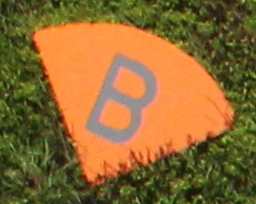
\includegraphics[width=0.4\textwidth]{target_example.jpg}
	\caption{Example Target}
	\label{fig:example_target}
\end{figure}

Figure~\ref{fig:example_target} shows an example target taken from real target imagery during UCSD AUVSI's 2013 competition flight. The characteristics of this target are easily identifiable using human visual identification, but autonomous computer identification of the same target can be a significant challenge to overcome. In the following sections we will describe the design and implementation of the NUAUVSI system.

\section{High-Level Overview}

NUAUVSI is designed with several goals in mind: 
 
\begin{description}
\item[Accuracy] Without accurate and reliable target characteristics, the basic goals of the competition would not be accomplished
\item[Performance] A fast system is required to analyze the high volume of imagery within a reasonable timespan
\item[Autonomy] The system must be able to run without human interaction in order to qualify as being `autonomous'
\item[Modularity] The ability to switch out certain CV algorithms for others is critical to ensure the longevity and maintainability of the system
\item[Cross-Platform] In order to be run from any computer we choose, the system needed to be able to be run on any major OS, and use only multi-platform libraries
\item[Simplicity] The system should, to within a reasonable degree, be implemented as simply as possible in order to increase maintainability and usefulness
\end{description}

The system we developed uses a distributed model to process imagery. This means that multiple computers can simultaneously work together to analyze the incoming imagery. This design model addresses several of our goals at once:

\begin{itemize}
\item[-] Multiple computers allows us to parallelize our computation until its speed of execution suits our needs
\item[-] Modular design naturally suits a model where different modules can run on different computers
\item[-] A distributed system should be cross-platform in order to increase to number of computers that can aid in computation
\end{itemize}
NUAUVSI can logically be split into three separate portions: the Backbone, the CV, and the GUI.

\subsection{Backbone}

\subsection{Computer Vision}

\subsection{GUI}

\section{Low-Level Description}

\subsection{Backbone}

\subsection{Computer Vision}

\subsection{GUI}

\section{Code Structure and Repository Information}

\section{List of Technologies Used}

\end{document}